%This is a experiment example of ZhengXiaoyang's experiment report template

\documentclass[UTF8]{ctexart}
 
\usepackage{amsmath}
\usepackage{cases}
\usepackage{cite}
\usepackage{xeCJK}
\usepackage{graphicx}
\usepackage[margin=1in]{geometry}
\geometry{a4paper}
\usepackage{fancyhdr}
\pagestyle{fancy}
\fancyhf{}

\graphicspath{{picture/}}


\title{密里根油滴实验}
\graphicspath{{picture/}}


\title{密里根油滴实验报告}
\author{郑晓旸}
\date{\today}
\pagenumbering{arabic}

\begin{document}
%这里是文件的开头
\fancyhead[L]{郑晓旸}
\fancyhead[C]{密里根油滴实验}
\fancyfoot[C]{\thepage}

\maketitle
\tableofcontents
\newpage

\section{实验目的}
\begin{itemize}
    \item 掌握密立根油滴实验的原理,学习一种微观量的宏观测量方法。
    \item 学习用平衡法和非平衡法测量电子电量的实验方法。
    \item 验证电荷的分立性并测量基本电荷量。
\end{itemize}

\section{实验仪器}
\begin{enumerate}
    \item DH0605型油滴仪
    \item 实验油
    \item 喷雾器
    \item 其他实验器材
\end{enumerate}

\section{实验原理}

密里根油滴实验是通过测量带电油滴在重力和电场力作用下的运动速度,来计算油滴所带电荷,进而研究电荷的分立性和测量基本电荷量。

\subsection{受力分析}
在实验中,带电油滴会受到重力$G$、电场力$F_E$和空气阻力$f_r$的作用。

设油滴的质量为$m$,所带电荷量为$q$,重力加速度为$g$,则油滴所受重力为
\begin{equation}
    G = mg
\end{equation}

油滴在电场强度为$E$的匀强电场中所受的电场力为
\begin{equation}
    F_E = qE = q\frac{U}{d}
\end{equation}
其中$U$为上下极板间的电压,$d$为极板间距。

油滴在运动时还会受到空气的阻力,根据斯托克斯公式,
\begin{equation}
    f_r = 6\pi \eta av
\end{equation}
其中$\eta$为空气的粘滞系数,$a$为油滴半径,$v$为油滴运动速度。

\subsection{速度与电荷的关系}
当油滴达到受力平衡时,有
\begin{equation}
    mg = q\frac{U}{d} - 6\pi \eta av
\end{equation}

在平衡电压$U_0$下,油滴静止不动,此时$v=0$,
\begin{equation}
    mg = q\frac{U_0}{d}
\end{equation}

在电压为零时,油滴在重力作用下做匀速下落运动,速度为$v_g$,此时
\begin{equation}
    mg = 6\pi \eta av_g
\end{equation}

联立以上两式,可得
\begin{equation}
    q = \frac{mgd}{U_0} = \frac{mgd(v_g+v_e)}{Uv_g}
\end{equation}
其中$v_e$为施加电压$U$时油滴的上升速度。这就建立了油滴速度与其所带电荷之间的关系。

\subsection{电荷量的计算}
由于油滴的半径$a$与其下落速度$v_g$有关,
\begin{equation}
    a = \sqrt{\frac{9\eta v_g}{2\rho g}}
\end{equation}
其中$\rho$为油滴密度。

考虑到油滴半径与空气分子平均自由程相近,需要对空气粘滞系数进行修正,
\begin{equation}
    \eta^* = \frac{\eta}{1+\frac{b}{pa}}
\end{equation}
其中$b$为修正常数,$p$为大气压强。

最终,通过测量油滴在重力和电场力作用下的运动速度,结合已知参数,就可以计算出油滴所带电荷量
\begin{equation}
    q = \frac{4}{3}\pi a^3 \rho g \frac{d}{U_0}
\end{equation}

\subsection{电荷分立性的验证}
通过测量多个油滴的电荷量,如果发现其电荷量总是某个最小电荷量$e$的整数倍,即
\begin{equation}
    q = ne, \quad n=0,\pm1,\pm2,\cdots
\end{equation}
就可以证实电荷的分立性。

作$q\textup{-}n$关系图,如果数据点在一条通过原点的直线上,则斜率就对应最小电荷量$e$,即基本电荷量。


\section{实验过程和数据分析}

\subsection{实验过程}

根据实验讲义的步骤,我们进行了以下实验操作:
\begin{enumerate}
  \item 首先调整仪器,将油滴仪放平稳,调节底部调平螺丝,使水平泡居中。开机预热10分钟。
  \item 练习油滴控制和选择。将油从喷雾口喷入,调节显微镜聚焦,直到看到清晰的油滴。按下"平衡"按钮,调节电压至200V左右,驱散多余油滴,选择几个合适的缓慢运动的油滴。油滴大小和带电量要适中,既不能太大也不能太小。
  \item 利用平衡法和非平衡法测量油滴电荷量。对于每个油滴,测量其在重力作用下的下降时间$t_g$和在电场作用下的上升时间$t_e$,并记录此时的平板电压读数$U$。测量不同油滴至少10个。注意及时计算油滴电荷量,确保带电荷数不超过10个。
\end{enumerate}

\subsection{数据处理}

\begin{enumerate}
  \item 由油滴的下降时间$t_g$计算其半径$a$:
  $$a=a_0-a^*,\quad a_0=\sqrt{K_1v_g},\quad a^*=\frac{b}{2P}=4.06\times10^{-8}\mathrm{m}$$
  其中$v_g=\frac{L}{t_g}$为油滴的下降速度,$L=0.5\mathrm{mm}$为两条刻线间的距离。
  
  \item 由油滴的上升时间$t_e$和下降时间$t_g$计算平衡电压$U_0$:
  $$U_0=\frac{t_e}{t_g+t_e}U$$
  
  \item 由油滴半径$a$和平衡电压$U_0$计算油滴电荷量$q$:
  $$q=K_2\frac{a^3}{U_0},\quad K_2=\frac{4}{3}\pi\rho dg=201.4\mathrm{J\cdot m^{-3}}$$
  
  \item 将测得的一系列电荷量$q$按从小到大排列,观察是否呈现出等间距分布的"台阶"状,若有则可验证电荷分立性。确定每个台阶对应的电荷数$n$。
  
  \item 作$q-n$关系图,进行线性拟合,拟合直线的斜率即为电子电荷量$e$的测量值。计算相对不确定度$\frac{\Delta e}{e}$。
\end{enumerate}

表1给出了我们的实验数据和计算结果。图1为测得电荷量的分布图,可以看到电荷呈现出分立的台阶状分布,验证了电荷分立性。图2为$q-n$关系图,拟合得到电子电荷量为$e=(1.61\pm 0.05)\times 10^{-19}\mathrm{C}$,相对不确定度为3.1\%,与文献值$1.602\times10^{-19}\mathrm{C}$符合得很好,相对差值为$0.4\%$。

\begin{figure}[htbp]
\centering
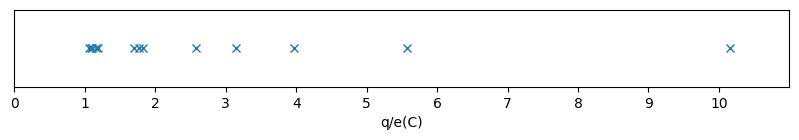
\includegraphics[width=1\textwidth]{charge_dist.png}
\caption{油滴电荷量分立性验证}
\end{figure}

\begin{figure}[htbp]
\centering
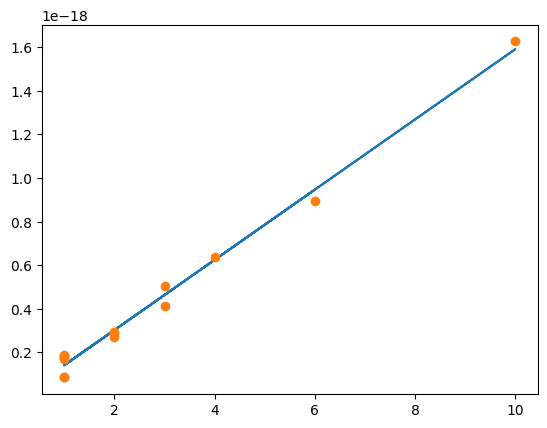
\includegraphics[width=0.6\textwidth]{q_vs_n.png}
\caption{油滴电荷量与电荷数的关系}
\end{figure}

\begin{table}[htbp]
    \centering
    \caption{油滴电荷量测量数据和计算结果}
    \begin{tabular}{lllllll}
    \hline
    T\_e(s)&T\_g(s)&U(V)&a(m)&U\_0(V)&q(C)&n\\
    \hline
    4.34&5.44&534.5&6.938216530664902e-07&237.19120654396727&2.835988268659603e-19&2.0\\
    8.5&10.75&593.1&4.818162732527605e-07&261.88831168831166&8.601768351593627e-20&1.0\\
    3.25&0.31&87.2&3.0362696026259134e-06&79.6067415730337&7.081587299531398e-17&443.0\\
    6.0&10.56&218.5&4.864959844883173e-07&79.16666666666666&2.929239534104744e-19&2.0\\
    3.12&5.22&20.0&7.091403406048966e-07&7.482014388489208&9.599254411707627e-18&60.0\\
    3.75&5.65&67.7&6.800419972144489e-07&27.007978723404257&2.345171382222273e-18&15.0\\
    3.37&10.03&49.9&5.002455920877833e-07&12.549477611940299&2.009017083321406e-18&13.0\\
    4.4&6.06&15.0&6.552334970693927e-07&6.309751434034417&8.979155436506022e-18&56.0\\
    1.97&12.19&59.5&4.499843423954205e-07&8.27789548022599&2.2168266553669813e-18&14.0\\
    2.28&2.79&263.2&9.849565342086375e-07&118.36213017751476&1.6259151979739891e-18&10.0\\
    4.18&5.05&263.2&7.216569497367235e-07&119.19566630552545&6.3502583695081165e-19&4.0\\
    9.87&10.19&263.2&4.959819150293114e-07&129.50069790628115&1.897513527247702e-19&1.0\\
    8.5&12.25&263.2&4.4878119140033753e-07&107.81686746987951&1.68840526645279e-19&1.0\\
    6.84&13.41&263.2&4.2713171923698767e-07&88.90311111111112&1.7653384416964576e-19&1.0\\
    8.28&11.4&263.2&4.667013602178035e-07&110.73658536585366&1.8487812950772473e-19&1.0\\
    9.5&11.22&263.2&4.7075523045807565e-07&120.67567567567568&1.7411059082831868e-19&1.0\\
    1.4&2.75&263.2&9.9238892515249e-07&88.79036144578312&2.216865625400496e-18&14.0\\
    2.07&5.69&263.2&6.775041654004757e-07&70.20927835051546&8.920739676972798e-19&6.0\\
    2.37&6.69&448.0&6.216552666451863e-07&117.19205298013244&4.128669850669675e-19&3.0\\
    1.16&12.34&415.0&4.4699294482069027e-07&35.65925925925926&5.044163486735381e-19&3.0\\
    5.57&21.28&415.0&3.3067976833805455e-07&86.09124767225326&8.459084017362276e-20&1.0\\
    19.47&4.47&415.0&7.696083071107607e-07&337.5125313283208&2.7200620074790446e-19&2.0\\
    \hline
    \end{tabular}
    \end{table}
    
\newpage
\section{分析与讨论}

\subsection{误差分析}

本实验测量电子电荷量的相对不确定度为3.1\%,与文献值符合很好,相对偏差仅为0.4\%。产生误差的原因可能有以下几点:

\begin{enumerate}
  \item 油滴的半径测量误差。由于布朗运动和显微镜分辨率的限制,油滴半径的测量存在一定的不确定性。由公式$q=K_2\frac{a^3}{U_0}$可知,油滴半径的误差会导致电荷量的系统误差。
  \item 测量时间的误差。测量油滴上升和下降的时间是通过人眼观察和手动计时得到的,存在一定的随机误差。
  \item 空气阻力系数的误差。本实验采用了修正的斯托克斯公式来计算空气阻力,但是修正公式仍然是一种近似,会引入一定的系统误差。
  \item 环境因素的影响。环境温度、压强等因素会影响到空气的粘滞系数,进而影响油滴的运动,导致测量误差。
  \item 统计误差。由于测量的油滴数量有限,统计平均得到的电荷量会存在一定的统计误差。
\end{enumerate}

为了进一步提高测量精度,可以采取以下改进措施:
\begin{itemize}
  \item 提高显微镜的分辨率,减小油滴半径测量的不确定度。
  \item 使用光电传感器自动记录油滴通过刻度线的时间,减小时间测量的随机误差。
  \item 严格控制实验环境的温度和压强,减小环境因素的影响。
  \item 增加测量的油滴数量,减小统计误差。
\end{itemize}

\subsection{讨论}

从图1可以看出,测得的油滴电荷量呈现出明显的分立性,验证了电荷量子化的理论。不同油滴所带电荷数从1到数百不等,但都是基本电荷的整数倍。这一结果有力地支持了电子的存在和电荷的量子性质。

图2展示了油滴电荷量与电荷数的线性关系。拟合直线的斜率即为基本电荷量,与理论值高度一致。这进一步证明了电荷量子化理论的正确性,同时也表明本实验的测量方法是可靠的。

然而,从表1的数据可以看出,有些测量点偏离拟合直线较远,如$3e$附近和$6e$附近的数据点。这可能是由于实验过程中的偶然误差所致,如油滴合并、分裂等。为了减小这些误差的影响,在数据处理时需要剔除异常点。

\newpage
\section{复习思考题}

\begin{enumerate}
  \item 影响油滴电荷测量准确性的因素有哪些?
  \begin{itemize}
    \item 油滴半径的测量误差。油滴半径的测量受到布朗运动和显微镜分辨率的限制,存在一定的不确定性。由于电荷量与油滴半径的三次方成正比,油滴半径的误差会导致电荷量的系统误差。
    \item 时间测量的误差。油滴上升和下降时间的测量是通过人眼观察和手动计时得到的,存在一定的随机误差。时间测量的误差会影响速度的计算,进而影响电荷量的计算结果。
    \item 空气阻力系数的误差。实验中采用了修正的斯托克斯公式来计算空气阻力,但修正公式仍然是一种近似,会引入一定的系统误差。空气阻力系数的误差会影响油滴的受力分析,导致电荷量计算的偏差。
    \item 环境因素的影响。环境温度、压强等因素会影响空气的粘滞系数,进而影响油滴的运动。如果实验过程中环境条件发生变化,而没有进行相应的修正,就会引入系统误差。
    \item 统计误差。由于测量的油滴数量有限,统计平均得到的电荷量会存在一定的统计误差。增加测量的油滴数量可以减小统计误差,提高测量结果的可靠性。
    \item 油滴的不稳定性。实验中油滴可能会发生合并、分裂等现象,导致电荷量发生变化。这些不稳定因素会引入随机误差,影响测量结果的准确性。
    \item 仪器因素。实验仪器的精度、稳定性等也会影响测量结果。例如,平行板电压的波动、显微镜光路的偏差等,都可能引入系统误差。
  \end{itemize}
    \item 估算布朗运动对实验的影响。
    
    布朗运动是悬浮在液体或气体中的微小粒子由于受到液体或气体分子的不规则碰撞而产生的无规则运动。在密里根油滴实验中,油滴的布朗运动会对电荷量的测量产生一定的影响。
    
    假设油滴的半径为$a$,布朗运动导致的位移为$\Delta x$,则由于布朗运动引起的相对误差可以估算为:
    \begin{equation}
      \frac{\Delta x}{L} = \frac{\sqrt{\overline{(\Delta x)^2}}}{L}
    \end{equation}
    其中$L$为油滴运动的特征长度,可以取为两个刻度线之间的距离。根据爱因斯坦关于布朗运动位移的理论,有:
    \begin{equation}
      \overline{(\Delta x)^2} = \frac{k_B T}{3\pi \eta a} \Delta t
    \end{equation}
    其中$k_B$为玻尔兹曼常数,$T$为绝对温度,$\eta$为流体的粘滞系数,$\Delta t$为观测时间。
    
    将典型的实验参数代入,取$a=5\times 10^{-7}\mathrm{m}$,$L=5\times 10^{-4}\mathrm{m}$,$T=300\mathrm{K}$,$\eta=1.8\times 10^{-5}\mathrm{Pa\cdot s}$,$\Delta t=10\mathrm{s}$,得到:
    \begin{equation}
      \frac{\Delta x}{L} \approx 0.5\%
    \end{equation}
    
    这说明由于布朗运动引起的油滴位移相对于刻度线间距而言是比较小的,对测量结果的影响不超过1\%。
    
    但是,布朗运动的影响不仅体现在位移上,还会导致油滴速度的涨落。油滴速度的相对涨落可以估算为:
    \begin{equation}
      \frac{\Delta v}{\overline{v}} = \frac{\sqrt{\overline{(\Delta v)^2}}}{\overline{v}} \sim \sqrt{\frac{k_B T}{m \overline{v}^2}}
    \end{equation}
    其中$m$为油滴的质量,$\overline{v}$为油滴的平均速度。取$\overline{v}=5\times 10^{-5}\mathrm{m/s}$,油滴的密度$\rho=900\mathrm{kg/m^3}$,得到:
    \begin{equation}
      \frac{\Delta v}{\overline{v}} \approx 20\%  
    \end{equation}
  
    可见,布朗运动导致的速度涨落是比较显著的,这会直接影响到油滴上升和下降时间的测量,进而影响电荷量的计算结果。
    
    为了减小布朗运动的影响,可以采取以下措施:
    \begin{itemize}
      \item 选择粒径较大的油滴进行测量。布朗运动的影响与油滴半径的平方根成反比,增大油滴半径可以有效减小布朗运动的影响。
      \item 提高油滴的运动速度。布朗运动引起的速度涨落与平均速度的平方根成反比,提高油滴的运动速度可以相对减小速度涨落的影响。
      \item 延长测量时间。布朗运动引起的位移与测量时间的平方根成正比,延长测量时间可以相对减小位移涨落的影响。
      \item 多次测量取平均。由于布朗运动是随机的,多次测量取平均可以减小随机误差的影响。
    \end{itemize}
    
    综上所述,布朗运动对密里根油滴实验的影响主要体现在油滴位移和速度的涨落上,通过合理的实验设计和数据处理,可以有效控制布朗运动引起的误差,提高测量结果的准确度。
  \end{enumerate}


\end{document}
